\documentclass{article}

\textwidth=6.5in
\textheight=8.5in
\voffset=-54pt
\oddsidemargin=0in
\evensidemargin=0in
\setlength{\parskip}{8pt}
\setlength{\parindent}{0pt}

\usepackage{workbook}

\usepackage{handout}

\usepackage{exam}

\newcommand{\answerbox}[3][]{
    \fbox{\begin{minipage}[t][#2][c]{#3}
        #1
    \end{minipage}}
    }

\begin{document}

{\large \mbox{} \hfill \bf Name:\underline{\hspace{3in}}}\\[2pt]
{\mbox{} \hfill \it (Please write your name neatly in print.)}\\[12pt]
{\large \mbox{} \hfill \bf HUID:\underline{\hspace{3in}}}
 
\medskip
 
\noindent
{\large\bf
Exam 1\\
Math Mb Spring 2025}
\noindent


{\Large
\begin{center}\textbf{Directions---Please read carefully!} \end{center}}


This exam is subject to the Harvard College Honor Code. No calculators or any other aids are permitted.  Please write as neatly as possible, as answers that can't be read can't be graded and thus can't receive credit. To receive full credit, you must show relevant working
and include units when appropriate. 

You have 120 minutes to complete this exam. 

You may ask for scratch paper if you need additional space to write, but it will not be scanned or graded. Make sure to include all relevant working in this exam booklet in the space provided for each question.

\begin{center}\textbf{Good luck!}\end{center}


\vfill

\centering{
\emph{As a member of Harvard College, I pledge that I will not give or receive assistance on this exam.}}
\vspace{0.3in}

{\large \mbox{} \hfill \bf Signature:\underline{\hspace{3in}}}
\thispagestyle{empty}

\newpage

\begin{enumerate}

\item
\begin{problem}
Luke needs help finding the derivatives of these functions! You do not need to simplify your answers.
\end{problem}

\begin{enumerate}

    \item 
    \begin{problem}
        % $f(x)=\pi \sin^2(x)\cos(x^2)$
        $f(x)=\pi \sin^2(x)$
    \end{problem}
    \pspace{\stretch{1}}

    \item 
    \begin{problem}
        % $g(x)=x\sec x + \arccos x$
        $g(x)=\csc(e^x) + \arcsin (e^x)$
    \end{problem}
    \pspace{\stretch{1}}
    
    \item 
    \begin{problem}
        % h(x) = x^{\arctan x}
        $h(x)=x^{\ln x}$
    \end{problem}
    \pspace{\stretch{1}}

\end{enumerate}

\newpage

\item 
\begin{problem}
    Yana has programmed a camera drone to follow the curve shown below (called a trifolium) as it flies. The equation of the curve is 
    \[(x^2+y^2)^2 = -2(x^3-3xy^2)\]
\end{problem}
\vspace{-16pt}
\begin{enumerate}[topsep=0pt]
    \item 
    \begin{problem}
        Find an equation for the line tangent to the curve at the point $(1, 1)$. Make sure your answer is consistent with the graph shown below.
        
        
\includegraphics[width=2in]{assessments/Exam 1/Exam1_Trifolium.png}
    \end{problem}
    \pspace{\vfill}
    \end{enumerate}

    \pspace{\newpage}
    
    \begin{framed}
        Continued from the previous page. The problem statement and graph are provided again below.
    
   Yana has programmed a camera drone to follow the curve shown below (called a trifolium) as it flies. The equation of the curve is 
    \((x^2+y^2)^2 = -2(x^3-3xy^2)\).
    \begin{center}
            
\includegraphics[width=2in]{assessments/Exam 1/Exam1_Trifolium.png}
            \end{center}
    \end{framed}
    
    \begin{enumerate}[resume]
    \item 
    \begin{problem}
        Yana's camera drone has just passed the point $(1, 1)$, and its $x$-coordinate is currently $0.9$. Use linear approximation to estimate its current $y$-coordinate. 
    \end{problem}
    \pspace{\stretch{0.5}}

    \item 
    \begin{problem}
        The drone's $x$-coordinate IS / IS NOT (circle one) a function of its $y$-coordinate, because... (complete the justification.)
    \end{problem}
    \pspace{\stretch{0.5}}
\end{enumerate}

\pspace{\newpage}

% \item Anda has been given the following information about an angle $A$: $\frac{3\pi}{2}<A<2\pi$ and $\cos A = \frac{3}{8}$. 
%     \begin{enumerate}
%     \item Sketch the angle in standard position on the unit circle below.
    
%     \begin{tikzpicture}
%     \begin{axis}[xmin=-1.2,xmax=1.2,ymin=-1.2,ymax=1.2,
%     xlabel=$x$, ylabel=$y$,
%     width=3in, unit vector ratio*={1 1},
%     xtick={1}, ytick=\empty,clip=false,
%     x tick label style={xshift=3pt}]
%     \coordinate (O) at (0,0);
%     \coordinate (A) at (1,0);
%     \addplot[black,domain=0:360,data cs=polar] (x,1);
%     \solonly{
%     \draw[dashed] (axis cs:-0.6,-1.2) -- node[midway, below] {${-\frac{3}{5}}$} (axis cs:-0.6,1.2);
%     \addplot[closed] coordinates {(-0.6,0.8)};
%     \draw[very thick, ->] (axis cs: 0,0) -- (axis cs: 1.2,0);
%     \draw[very thick, ->] (axis cs: 0,0) -- (axis cs: -0.9, 1.2);
%     \addplot[domain=0:126.9,->] ({0.2*cos(x)},{0.2*sin(x)});
%     \node at (axis cs: 0.15, 0.25) {$\theta$};
%     }
%     \end{axis}
%   \end{tikzpicture}

%   \item Help Anda find the values of the following expressions. If an expression is undefined, write ``undefined."
%   \begin{tasks}[label=\roman*.,after-item-skip=120pt, label-width=12pt](2)
%         \task $\cos (-A)$
%         \task $\cos (\pi + A)$
%         \task $\sin A$
%         \task $\cos^2 A + \sin^2 A$
%         \task $\cos(\arccos A)$
%         \task $\arccos(\cos A)$
%   \end{tasks}
    
% \end{enumerate}
% \pspace{48pt}

% \item Decide whether each statement is true \textbf{for all values $x$ for which the expressions are defined}. You do not need to consider values for which the expressions are not defined. Fill in the appropriate bubble. No explanation is necessary.

% \begin{minipage}{2.5in}
% \begin{enumerate}\tfheading

% \item\begin{tf}{f} $\cos(x)=\cos(x+\pi)$
% \end{tf}

% \item\begin{tf}{f} $\cos(\arccos(x))=x$ \vphantom{$\dfrac{1}{\tan(x)}$}
% \end{tf}

% \item\begin{tf}{f} $\arccos(\cos(x))=x$ \vphantom{$\dfrac{x}{x}$}
%  \end{tf}
% \end{enumerate}
% \end{minipage}
% \hspace{2cm}
% \begin{minipage}{2.5in}
% \begin{enumerate}[start=4]\tfheading
% \item\begin{tf}{f} $-\tan(x)=\tan(-x)$  
%  \end{tf}
 
% \item\begin{tf}{f} $\dfrac{1}{\tan(x)}=\cot(x)$ 
%  \end{tf}

% \item\begin{tf}{f} $\dfrac{1}{\sin(x)}=\arcsin(x)$
%  \end{tf}

% \end{enumerate}
% \end{minipage}

\pspace{\newpage}

\item Matt needs help solving trig equations! For each equation, find all solutions on the interval $[0, 2\pi]$. Answer using special angles if possible, otherwise you may leave your answer in terms of inverse trigonometric functions. If there are no solutions, write ``no solution."

\begin{enumerate}[topsep=0pt]
    \item $\tan x =-0.4$
    \pspace{\vfill}

    \item $2\sin(2x)=\sqrt{3}$
    \pspace{\vfill}
    
    \item $2\sin(2x)=3$
    \pspace{\vfill}

    % \item $6\cos^2(x)-\cos(x)=1$\\ 
    % \pspace{\stretch{2}}
\end{enumerate}

\pspace{\newpage}

\item The temperature in a small desert village oscillates over a 24-hour period, with very high temperatures in the day and very low temperatures at night. Anda wants to model the temperature with a sinusoidal function $f(t)$, where $f(t)$ is measured in degrees Celsius, $t$ is measured in hours, and $t=0$ corresponds to midnight. Based on historical data, she makes the following assumptions: 
\begin{itemize}[nosep]
    \item The high temperature is $40\,^\circ$C and occurs at noon.
    \item The low temperature is $10\,^\circ$C and occurs at midnight.
\end{itemize} 
Answer the following questions based on Anda's model. 

\begin{enumerate}[topsep=0pt]
    \item Sketch the graph of $f(t)$ over one full 24-hour cycle, from $t=0$ to $t=24$. Label the axes, including units. On the axes, clearly label the midline value, maximum value, and minimum value, as well as the times when these three values are achieved.
    \pspace{\stretch{1}}
    
    \item Write a formula for $f(t)$.
    \pspace{\stretch{0.5}}
    
    \item Find the temperature at 6:00 PM ($t = 18$) by evaluating your formula from part (b). Simplify your answer fully and include units. Make sure this agrees with your sketch.
    \pspace{\stretch{1}}

    \pspace{\newpage}

    \end{enumerate}

\begin{framed}
        Continued from the previous page. The problem statement is provided again below.
    
   The temperature in a small desert village oscillates over a 24-hour period, with very high temperatures in the day and very low temperatures at night. Anda wants to model the temperature with a sinusoidal function $f(t)$, where $f(t)$ is measured in degrees Celsius, $t$ is measured in hours, and $t=0$ corresponds to midnight. Based on historical data, she makes the following assumptions: 
\begin{itemize}[nosep]
    \item The high temperature is $40\,^\circ$C and occurs at noon.
    \item The low temperature is $10\,^\circ$C and occurs at midnight.
\end{itemize} 
    \end{framed}

    \begin{enumerate}[resume]

    \item Find the time(s) between $t=0$ and $t=24$ when the temperature in the village is exactly $20\,^\circ$C. Give exact answers in terms of inverse trigonometric functions and include units.
    \pspace{\stretch{1}}

    \item Find $f'(t)$. 
    \pspace{\stretch{0.3}}



    \item State the maximum value of $f'(t)$. (You do not need to use calculus to find the maximum value.) Interpret the meaning of this value in the context of the problem. Include units.
    \pspace{\stretch{0.5}}

\end{enumerate}

\pspace{\newpage}

\item
Oxford Street and Kirkland Street form a right angle, and the Science Center is at the corner. Justin, Kate, and Sarah are chatting on the street corner. At 5:00 PM, Justin heads back into the Science Center, Kate starts walking away from the Science Center along Oxford Street at a speed of 4 ft/s, and Sarah starts walking away from the Science Center along Kirkland Street at a speed of 3 ft/s.


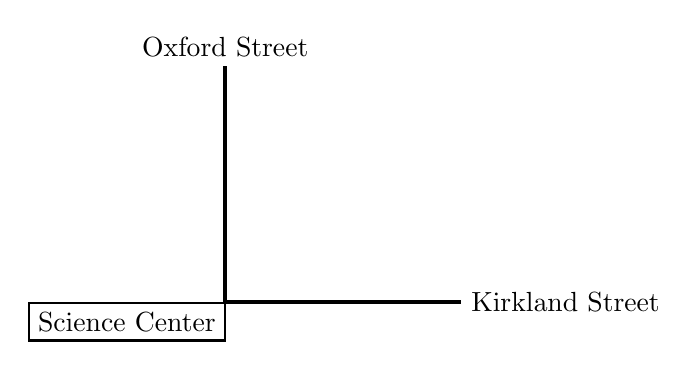
\begin{tikzpicture}

    % Draw the outlines of the streets
    \draw[ultra thick] (0, 0) -- (3, 0);
    \draw[ultra thick] (0,0) -- (0,3);

    % Label the streets
    \node[above] at (0, 3) {Oxford Street};
    \node[right] at (3, 0) {Kirkland Street};
    \node[draw, thick] at (-1.25,-0.25) {Science Center};
\end{tikzpicture}


\begin{enumerate}[topsep=0pt]
    \item Determine the distance between Kate and Sarah 10 seconds after 5:00 PM. Include units.
    \pspace{\stretch{0.5}}

    \item Determine how fast the distance between Kate and Sarah is increasing 10 seconds after 5:00 PM. Show all of the work that leads to your final answer. Include units.
    \pspace{\stretch{2}}
    
%     \item As Kate and Sarah walk away from the Science Center, does the distance between them increase faster and faster, slower and slower, or at a constant rate?  Circle one, no explanation necessary.
% \begin{enumerate}[label=\protect\maybecircle{\Alph*.}]
%     \plainitem Faster and faster
%     \circleitem Slower and slower
%     \plainitem At a constant rate
% \end{enumerate}
\end{enumerate}

\pspace{\newpage}

\item
Shanelle is modeling the population of deer in a large forest. The deer population goes up and down over time due to environmental factors. Shanelle decides to not use a sinusoidal model and instead chooses to model the population size with the function $P(t)=e^{2\cos t}$ graphed below. The function $P(t)$ represents the number of deer in thousands at time $t$, where $t$ is measured in years. 

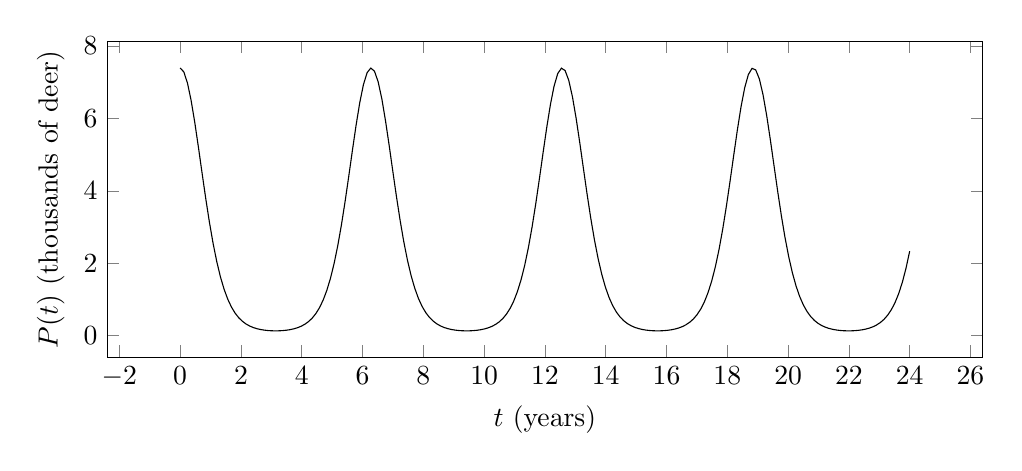
\begin{tikzpicture}
    \begin{axis}[
    xlabel=$t$ (years),
    ylabel={$P(t)$ (thousands of deer)},
    samples=200,
    height=2.2in,
    width=5in
    ]
        \addplot[domain=0:24] {e^(2*cos(deg(x))};
    \end{axis}
\end{tikzpicture}

\begin{enumerate}[topsep=0pt]
    \item Find the period of $P(t)$ and explain why $P(t)$ is a periodic function.
    \pspace{\stretch{1}}
        \item Based on Shanelle's model, what is the maximum number of deer in the forest? Give an exact value and include units. (This problem can be answered without using calculus. Show the work leading to your answer or explain your reasoning.)
    \pspace{\stretch{1.5}}

    \pspace{\newpage}

    % \item Write down the number of  times between $t=0$ and $t=6$ at which there are 4000 deer in the forest. No explanation needed.
    % \pspace{\stretch{0.25}}

    % \item Find the exact time(s) between $t=0$ and $t=6$ at which there are 4000 deer in the forest. Give exact answers in terms of logarithms and inverse trigonometric functions.
    % \pspace{\stretch{1}}
    
    % \item Find $\lim\limits_{t\to\infty} P(t)$. Explain your reasoning briefly.
    % \pspace{\stretch{.5}}
\end{enumerate}





\probonly{
\newpage
\textit{This page has been intentionally left blank for scratch work. No work on this page will be graded.}
}

\end{enumerate}
\end{document}